\section{Benchmarking the~AWBS nonlocal transport model}
\label{sec:BenchmarkingAWBS}
After having shown several encouraging properties of the~AWBS transport 
equation defined by \eqref{eq:AWBS_model} under local diffusive conditions
in \secref{sec:DiffusiveKinetics}, this section provides a~broader analysis
of the~electron transport and focuses on analysis its behavior under variety of
conditions in plasmas. In principle, this is characterized by allowing that
electron mean free path can be arbitrarily long, which leads to so-called 
nonlocal electron transport extensively investigated in numerous publications 
\cite{Malone_1975_15, Colombant_PoP2005, Bell_1981_83, LMV_1983_7, Brantov_Nonlocal_electron_transport_1998, schurtz2000, Sorbo_2015}, where the~Fokker-Planck
modeling of electrons in plasma represents the~essential tool. Being so, 
we introduce our implementation of the~AWBS transport equation called AP1,
where its results are further benchmarked against simulation results
provided by Aladin, Impact FP codes, and Calder a~collisional Particle-In-Cell
code. Their description follows in the~next section.

\begin{figure}[tbh]
  \begin{center}
    \begin{tabular}{c}
      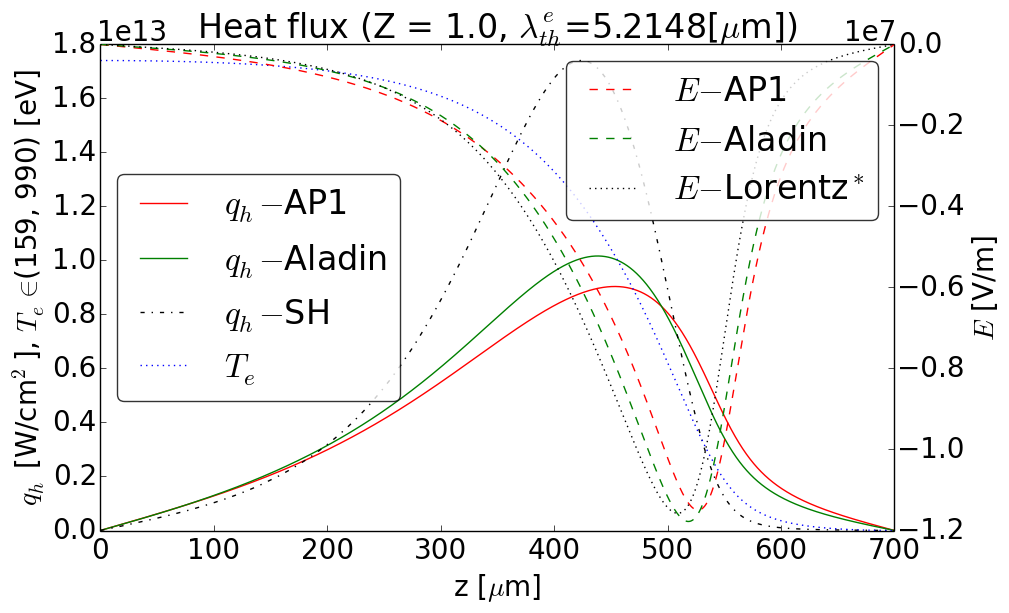
\includegraphics[width=\figscale\textwidth]{../VFPdata/C7_Aladin_case5_heatflux.png} \\
      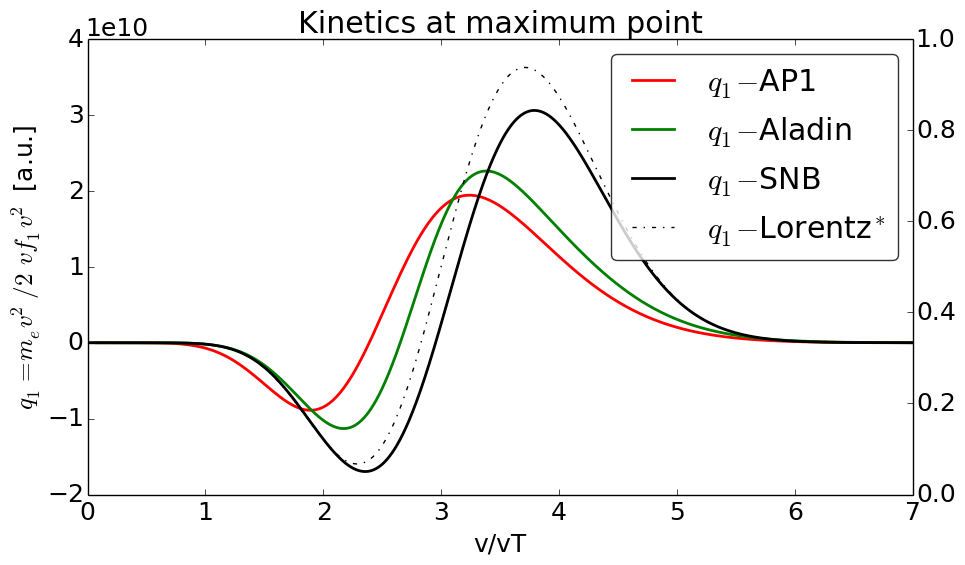
\includegraphics[width=\figscale\textwidth]{../VFPdata/C7_Aladin_case5_kinetics.png}
    \end{tabular}
  \caption{  
  Snapshot 20 ps. Left: correct steady solution of heat flux. 
  Right: Aladins results are correct. Velocity limit 4.4 $\vth$..
  }
  \label{fig:C7_Aladin_case5}
  \end{center} 
\end{figure}

\subsection{AP1 implementation}
\label{sec:C7code}

AP1 represents the~abbreviation AWBS-P1, i.e. the~use of collision operator 
\eqref{eq:AWBS_model} and the~P1 angular discretization, i.e. the~lowest order 
anisotropy approximation. AP1 in general belongs to the~so-called angular 
moments method and the~electron distribution function takes the~form
\begin{equation}
  \tilde{\ft} = \frac{\fzero}{4\pi} + \frac{3}{4\pi}\vn\cdot\fone , 
  \nonumber \label{eq:P1approximation}
\end{equation}
which consists of the~isotropic part $\fzero = \int_{4\pi} \tilde{\ft} \dI\vn$ 
and the~directional part $\fone = \int_{4\pi} \vn
\tilde{\ft} \dI\vn$, where $\vn$ is the~transport direction (the~solid angle).

The~first two angular moments applied to the~steady form of 
\eqref{eq:kinetic_equation} with collision operator \eqref{eq:AWBS_model} 
lead to the~AP1 model equations
\begin{eqnarray}
  \vmag\frac{\nue}{2}\pdv{}{\vmag}\left(\fzero - 4\pi\fM \right) &=&
  \vmag\nabla\cdot\fone + \tE\cdot
  \pdv{\fone}{\vmag} + \frac{2}{\vmag}\tE\cdot\fone , 
  \label{eq:AP1f0}\\
  \vmag\frac{\nue}{2}\pdv{\fone}{\vmag}
  - \nuscat\fone &=& 
  \frac{\vmag}{3}\nabla\fzero + 
  \frac{\tE}{3}\pdv{\fzero}{\vmag} ,
  \label{eq:AP1f1}
\end{eqnarray}
where $\nuscat = \nuei + \frac{\nue}{2}$. The~strategy of solving 
\eqref{eq:AP1f0} and \eqref{eq:AP1f1} resides in integrating 
$\pdv{\fzero}{\vmag}$
and $\pdv{\fone}{\vmag}$ in velocity magnitude while starting the~integration
from infinite velocity to zero velocity, which corresponds to decelerating 
electrons. It should be noted, that in practice we start the~integration from
$\vmag = 7 \vth$, which represents a~sufficiently high velocity.

\begin{figure}[tbh]
  \begin{center}
    \begin{tabular}{c}
      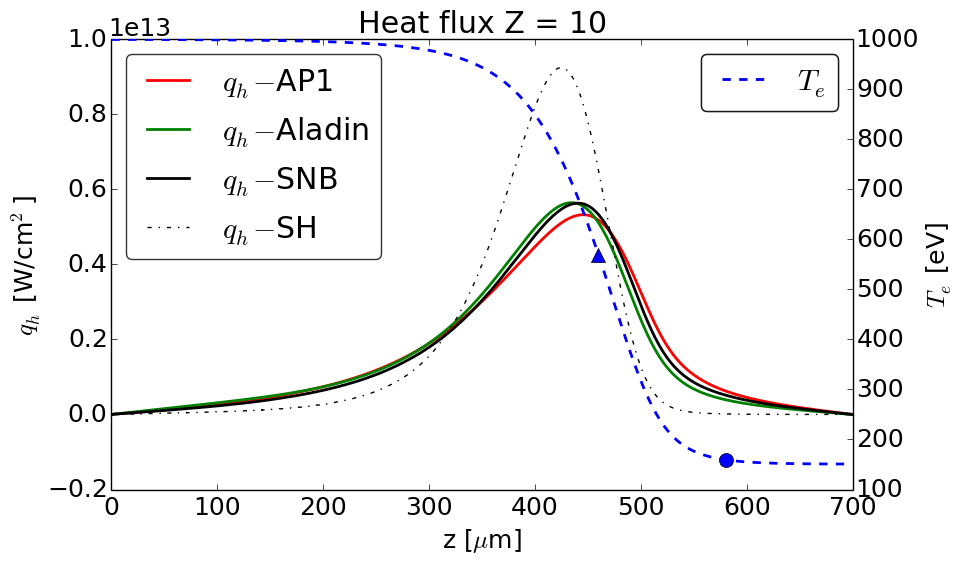
\includegraphics[width=\figscale\textwidth]{../VFPdata/C7_Aladin_case3_heatflux.png} \\
      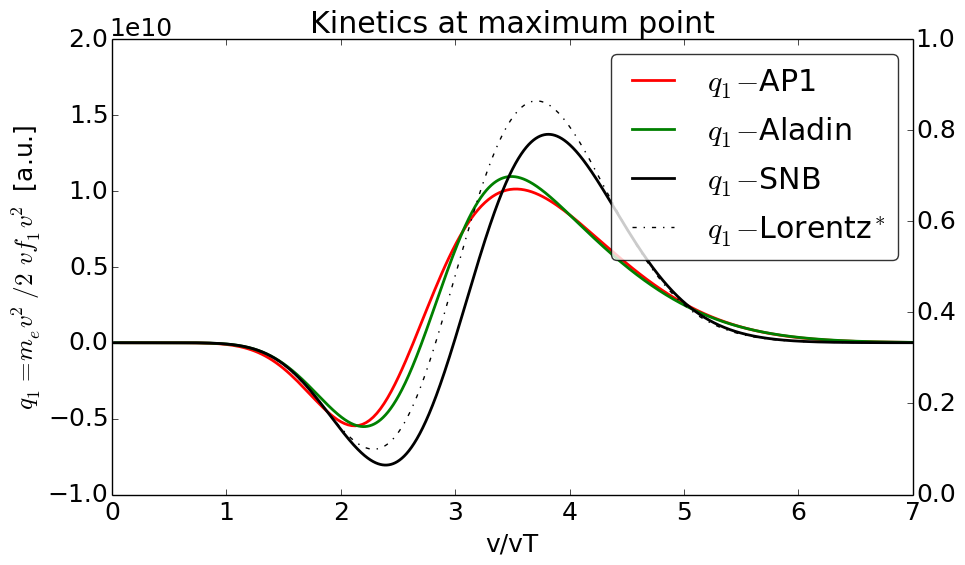
\includegraphics[width=\figscale\textwidth]{../VFPdata/C7_Aladin_case3_kinetics.png}
    \end{tabular}
  \caption{  
  Snapshot 12 ps. Left: correct steady solution of heat flux. 
  Right: correct comparison to kinetic profiles at point 442 $\mu$m by Aladin. 
  Velocity limit 3.4 $\vth$.
  }
  \label{fig:C7_Aladin_case3}
  \end{center} 
\end{figure}


\subsubsection{Nonlocal electric field treatment}
\label{sec:Efield}

%\begin{multline}
%  %\frac{\vect{j}}{\qe} = 
%  \vect{q}_c \equiv
%  \qe \intv \Bigg[\frac{\frac{\nue}{2}\vmag^2}{\nuei + \frac{\nue}{2}}
%  \pdv{\fone}{\vmag} 
%  - \frac{\vmag^2}{3\left(\nuei + \frac{\nue}{2}\right)}
%  \nabla\fzero \\
%  - \frac{\vmag}{3\left(\nuei + \frac{\nue}{2}\right)}\pdv{\fzero}{\vmag}\tE
%  \Bigg] \vmag^2\, \dI\vmag = 0
%  , \nonumber
%\end{multline}
Similarly to \eqref{eq:BGK_Efield}, one can obtain the~model equation of 
the~electric field $\tE$ by evaluating the~zero current condition 
(a~velocity integration of \eqref{eq:AP1f1})
\begin{equation}
  \intv \left(\frac{\frac{\nue}{2}\vmag^2}{\nuscat}
  \pdv{\fone}{\vmag} 
  - \frac{\vmag^2}{3\nuscat}
  \nabla\fzero 
  - \frac{\vmag}{3\nuscat}\pdv{\fzero}{\vmag}\tE
  \right) \vmag^2\, \dI\vmag = 0 ,
  \label{eq:AP1_Efield}
\end{equation}
from which it is easy to express $\tE$ once $\fzero$ and $\fone$ are known, or
in other words, the~integral-differential model equations need to be solved 
simultaneously, which is achieved by $k$-iteration of 
$\fzero^k(\tE^k), \fone^k(\tE^k)$, i.e. \eqref{eq:AP1f0}, \eqref{eq:AP1f1}, and 
$\tE^{k+1}(\fzero^k, \fone^k)$, i.e.  \eqref{eq:AP1_Efield}, until 
the~current evaluation \eqref{eq:AP1_Efield} converges to zero. In principle,
our concept of $k$-iteration resembles to the~embedded nonlinear iteration
of the~implicit E field introduced in \cite{Kingham_JCP2004}.
The~first iteration starts with $\tE=\vect{0}$ in \eqref{eq:AP1f0} and 
\eqref{eq:AP1f1} and usually less than 10 iterations is sufficient to obey
the~quasi-neutrality constraint.
%\begin{eqnarray}
%  \pdv{\fzero}{\vmag} &=&
%  \frac{2}{\nue}\pdv{\fonez}{z} + \frac{2\tEz}{\vmag\nue} \pdv{\fonez}{\vmag} 
%  + \frac{4}{\vmag^2\nue}\tEz\fonez 
%  + 4\pi\pdv{\fM}{\vmag}
%  , \nonumber\\
%  \vmag\frac{\nue}{2}\pdv{\fonez}{\vmag} 
%  &=&  
%  \frac{\tEz}{3}\pdv{\fzero}{\vmag} + \frac{\vmag}{3}\pdv{\fzero}{z} 
%  + \left(\nuei + \frac{\nue}{2}\right)\fonez
%  , \nonumber \label{eq:OOE_P1f1}
%\end{eqnarray}

Interestingly, we have encountered a~very specific property of the~AP1 model
with respect to the~electric field magnitude. The~easiest way how to 
demonstrate this is to write the~model equations \eqref{eq:AP1f0} and 
\eqref{eq:AP1f1} in 1D and eliminate one of the~partial derivatives with 
respect to $\vmag$. In the~case of elimination of $\pdv{\fzero}{\vmag}$ 
one obtains the~following equation
\begin{multline}
  %\frac{2}{3\vmag\nue} 
  %\left(\left(\sqrt{3}\vmag\frac{\nue}{2}\right)^2 - \tEz^2\right)  
  \left(\vmag\frac{\nue}{2} - \frac{2\tEz^2}{3\vmag\nue}\right) 
  \pdv{\fonez}{\vmag} 
  =
  \frac{2\tEz}{3\nue}\pdv{\fonez}{z}  
  + \frac{4\pi\tEz}{3}\pdv{\fM}{\vmag} \\
  + \frac{\vmag}{3}\pdv{\fzero}{z} 
  + \left(\frac{4\tEz^2}{3\vmag^2\nue}
  + \left(\nuei + \frac{\nue}{2}\right) \right)\fonez .
  \label{eq:AP1_model_1D}
\end{multline}
It is convenient to write the~left hand side of \eqref{eq:AP1_model_1D} as
$\frac{2}{3\vmag\nue} 
\left(\left(\sqrt{3}\vmag\frac{\nue}{2}\right)^2 - \tEz^2\right)$
from where it is clear that the~bracket is negative if 
$\sqrt{3}\vmag\frac{\nue}{2} =  \sqrt{3}\frac{n_e \Gamma}{2\vmag^2} < |\tE|$, 
i.e. there is a~velocity limit for a~given magnitude $|\tE|$, 
when the~collisions are no more fully dominant and the~electric field 
introduces a~comparable effect to friction in the~electron transport.

Since the~last term on the~right hand side of \eqref{eq:AP1_model_1D} 
is dominant, the~solution behaves as 
$\fone \sim \exp\left(-\left(\frac{4\tEz^2}{3\vmag^2\nue}
  + \left(\nuei + \frac{\nue}{2}\right) \right)/
\left(\vmag\frac{\nue}{2} - \frac{2\tEz^2}{3\vmag\nue}\right)\, \vmag\right)$, 
which becomes ill-posed for velocities above the~limit.

%\begin{table}
%\begin{center}
%  \begin{tabular}{c|ccccc}
%    \hline\hline\\
%    Kn$^e$ & $\,\,10^{-3}\,\,$ & $\,\,5\times10^{-3}\,\,$ & $\,\,10^{-2}\,\,$ & $\,\,5\times10^{-2}\,\,$ & $\,\,10^{-1}\,\,$ \\\\
%    \hline\\
%    $\vmag_{lim}^{Z=1} / \vth$ & 21.6 & 9.8 & 7.0 & 3.8 & 3.1 \\\\
%    \hline\\
%    $\vmag_{lim}^{Z=2} / \vth$ & 14.8 & 6.8 & 5.0 & 3.1 & 2.6 \\\\
%    \hline\\
%    $\vmag_{lim}^{Z=10} / \vth$ & 6.7 & 3.4 & 2.6 & 1.6 & 1.3 \\\\
%    \hline\hline
%  \end{tabular}
%  \caption{
%  $\sqrt{3}\vmag\frac{\nue}{2} > |\tE|$.
%  }
%\end{center}
%\label{tab:vlim}
%\end{table}

\begin{table}
\begin{center}
  \begin{tabular}{c|ccccc}
    \hline\hline\\
    %Kn$^e$ & $10^{-4}$ & $10^{-3}$ & $10^{-2}$ & $10^{-1}$ & $1$ \\\\
    Kn$^e$ & $\,\,10^{-4}\,\,$ & $\,\,10^{-3}\,\,$ & $\,\,10^{-2}\,\,$ & $\,\,10^{-1}\,\,$ & $\,\,1\,\,$ \\\\
    \hline\\
    $\vmag_{lim} / \vth$ & 70.8 & 22.4 & 7.3 & 3.1 & 1.8\\\\
    \hline\hline
  \end{tabular}
  \caption{
  $\sqrt{3}\vmag\frac{\nue}{2} > |\tE|$.
  }
\label{tab:vlim}
\end{center}
\end{table}

In order to provide a~stable model, we introduce a~reduced electric field
\begin{equation}
  |\tE_{red}| = \sqrt{3} \vmag\frac{\nue}{2} ,
  \label{eq:Elimit}
\end{equation}
ensuring that the~bracket on the~left hand side of \eqref{eq:AP1_model_1D}
remains positive. Further more we define two quantities
\begin{equation}
  \omega_{red} = \frac{|\tE_{red}|}{|\tE|} ,\quad 
  \nuscat^E = \frac{|\tE| - |\tE_{red}|}{\vmag} .
  \nonumber
\end{equation}
introducing the~reduction factor of the~electric field
$\omega_{red}$ and the~compensation of the~electric field effect in terms of
scattering $\nuscat^E$. Consequently, the~AP1 model \eqref{eq:AP1f0}, 
\eqref{eq:AP1f1}, and \eqref{eq:AP1_Efield} can be formulated as well posed 
with the~help of $\omega_{red}$ and $\nuscat^E$. However, before doing so,
we introduce a~slightly different approximation to the~electron distribution 
function as
\begin{equation}
  \tilde{f} = \frac{4\pi \fM + \dafzero}{4\pi} + \frac{3}{4\pi}\vn\cdot\fone .
  \label{eq:P1_OOE}
\end{equation}
where $\dafzero$ represents the~departure of isotropic part from 
the~Maxwell-Boltzmann equilibrium distribution $\fM$. 
%which we keep 
%intentionally in the~distribution function approximation.
Then, the~stable AP1 model reads
\begin{eqnarray}
  \vmag \frac{\nue}{2}\pdv{\dafzero}{\vmag} &=&
  \vmag\nabla\cdot\fone + \tE\cdot\left(\omega_{red} \pdv{\fone}{\vmag} 
  + \frac{2}{\vmag}\fone\right) , 
  \label{eq:AP1f0_stable}\\
  \vmag\frac{\nue}{2}\pdv{\fone}{\vmag} 
  &=& \tnuscat\fone 
  + \frac{\vmag}{3}\nabla\left(4\pi\fM + \dafzero\right)
  \nonumber \\
  && 
  + \frac{\tE}{3}\left(4\pi \pdv{\fM}{\vmag} 
  + \omega_{red} \pdv{\dafzero}{\vmag} 
  \right) ,
  \label{eq:AP1f1_stable}
\end{eqnarray}
where $\tnuscat = \nuei + \nuscat^E + \frac{\nue}{2}$.
The~reason for keeping $\fM$ in the~distribution function approximation
\eqref{eq:P1_OOE} can be seen in the~last term on the~right hand side of 
\eqref{eq:AP1f1_stable}, which provides the~effect of electric field on
directional quantities as current or heat flux. In principle, the~explicit use
of $\fM$ ensures the~proper effect of $\tE$ if $\dafzero \ll \fM$, i.e.
no matter what the~reduction $\omega_{red}$ is. Apart from its stability,
it also exhibits much better convergence of the~electric field, which is now
given by the~zero current condition of \eqref{eq:AP1f1_stable} as
\begin{equation}
  \tE =
  \frac{\intv \left(\frac{\nue}{2\tnuscat}\vmag^2\pdv{\fone}{\vmag}
  - \frac{\vmag^2}{3\tnuscat}
  \nabla\left(4\pi\fM + \dafzero\right)\right) \vmag^2\, \dI\vmag}
  {\intv \frac{\vmag}
  {3\tnuscat}
  \left(4\pi\pdv{\fM}{\vmag} + \omega_{red} \pdv{\dafzero}{\vmag}\right)
  \vmag^2\, \dI\vmag} .
  \label{eq:AP1_Efield_stable}
\end{equation}

For practical reasons we present in \tabref{tab:vlim} 
some explicit values of velocity limit corresponding to varying transport 
conditions expressed in terms of Knudsen number 
$\text{Kn}^e = \frac{\mfpe |\nabla T_e|}{T_e}$, 
where $\frac{T_e}{|\nabla T_e|}$ stands for the~length scale of plasma.

\begin{figure}[tbh]
  \begin{center}
    \begin{tabular}{c}
      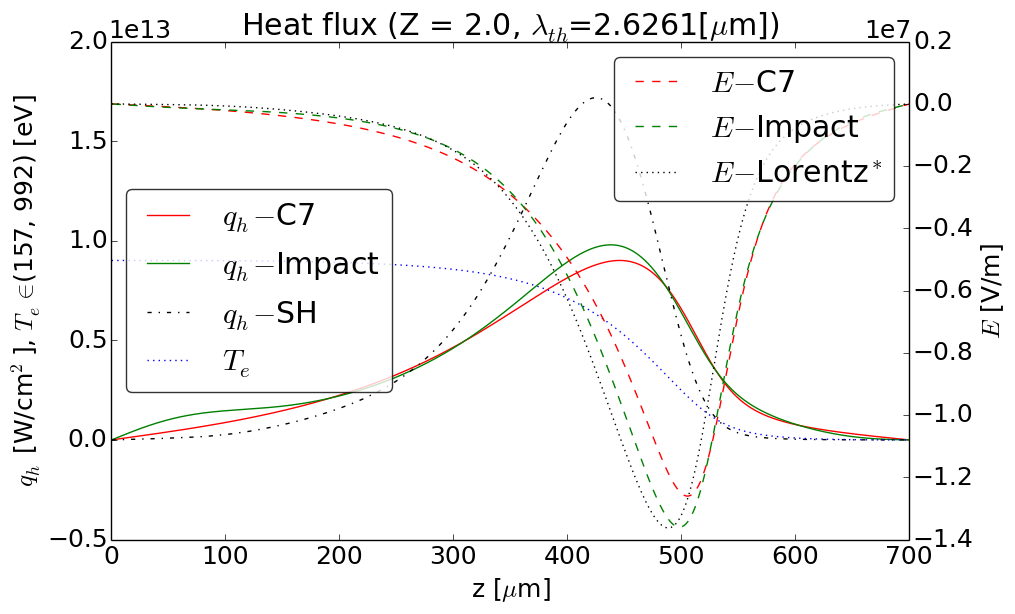
\includegraphics[width=\figscale\textwidth]{../VFPdata/C7_Impact_case3_heatflux.png} \\
      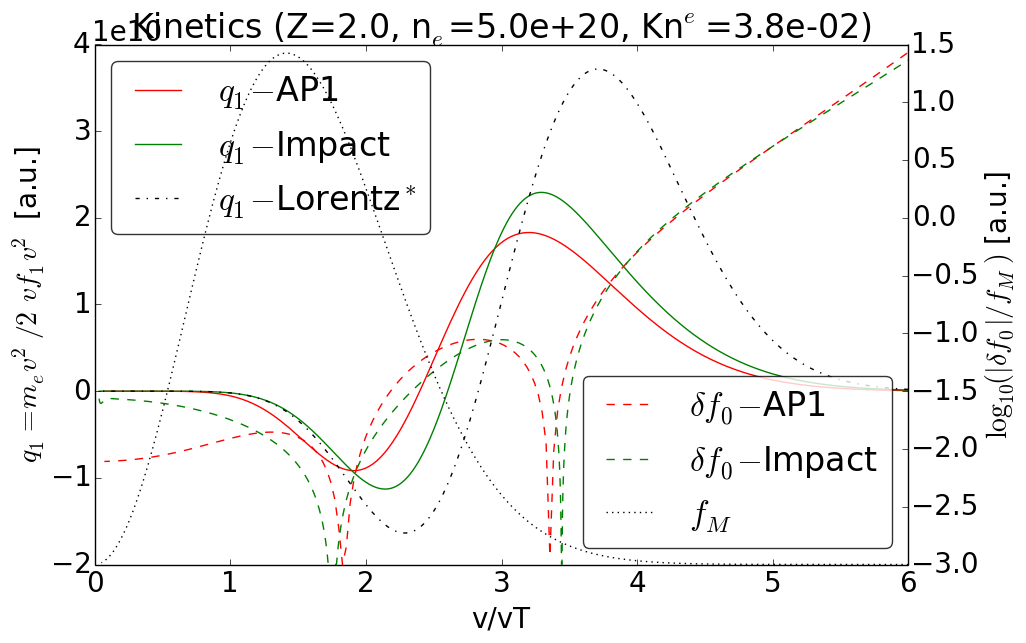
\includegraphics[width=\figscale\textwidth]{../VFPdata/C7_Impact_case3_kinetics.png}
    \end{tabular}
  \caption{  
  Snapshot 12 ps. Left: correct steady solution of heat flux. 
  Right: correct comparison to kinetic profiles at point 437 $\mu$m by Impact.
  Velocity limit 4.0 $\vth$.
  }
  \label{fig:C7_Impact_case3}
  \end{center} 
\end{figure}

\subsection{Aladin, Impact, and Calder kinetic codes}
\label{sec:AladinImpactCaldercodes}

\begin{itemize}
  \item Brief description of the Aladin code \figref{fig:C7_Aladin_case5}, \figref{fig:C7_Aladin_case3}. %\figref{fig:C7_Aladin_case6}
\end{itemize}

\begin{itemize}
  \item Brief description of the Impact code \figref{fig:C7_Impact_case3}.
\end{itemize}

\begin{figure}[tbh]
  \begin{center}
    \begin{tabular}{c}
      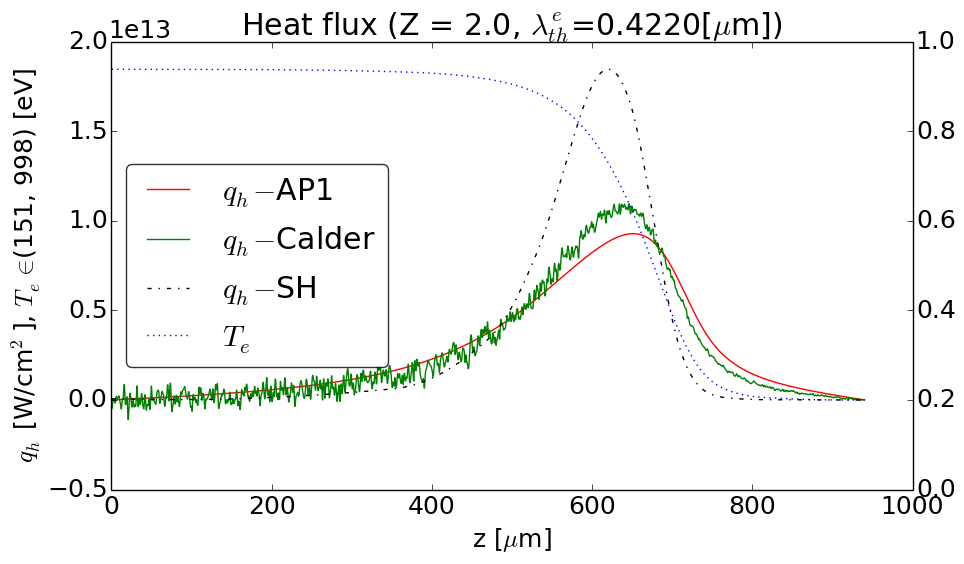
\includegraphics[width=\figscale\textwidth]{../VFPdata/C7_Calder_case1_heatflux.png} 
	  %\\ 
	  %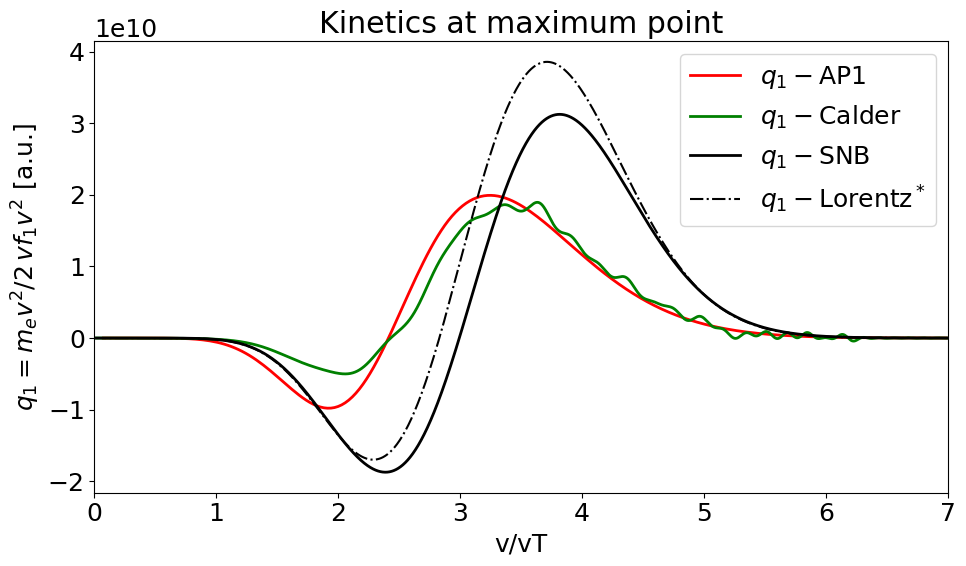
\includegraphics[width=\figscale\textwidth]{../VFPdata/C7_Calder_case1_kinetics.png}
    \end{tabular}
  \caption{  
  Snapshot 11 ps. Left: correct steady solution of heat flux. 
  %Right: AP1 kinetic profiles at point 750~$\mu$m corresponding to 
  %a~highly nonlocal nature of the~heat flux and is in a~good agreement with
  %\cite{Sherlock_PoP2017}. Velocity $max(q_1)$ = 5.8 $\vth$. 
  Velocity limit 6.4 $\vth$.
  }
  \label{fig:C7_Calder_case1}
  \end{center} 
\end{figure}

\begin{itemize}
  \item Brief description of the Calder code \figref{fig:C7_Calder_case1}.
\end{itemize}

\begin{figure}[tbh]
  \begin{center}
    \begin{tabular}{c}
	  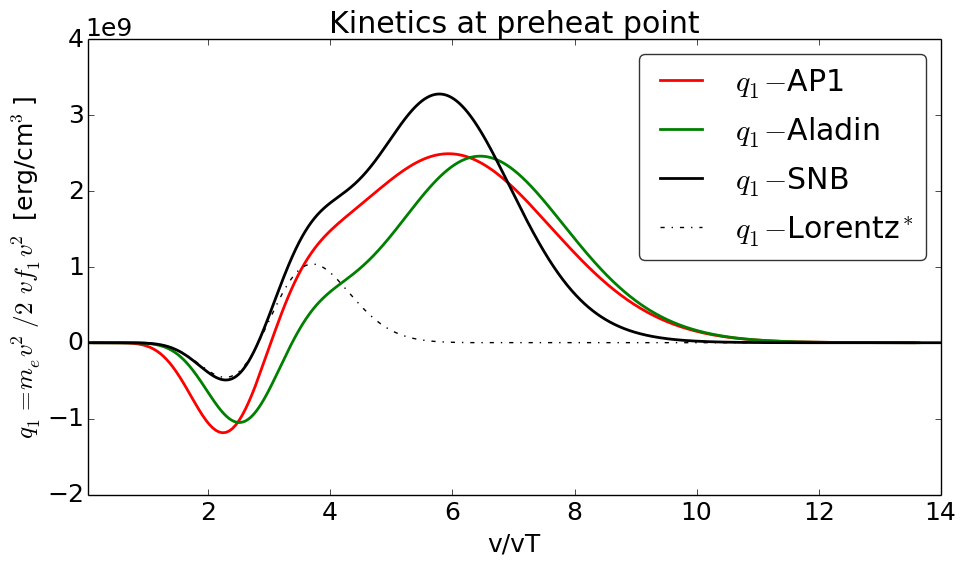
\includegraphics[width=\figscale\textwidth]{../VFPdata/C7_Aladin_case5_nonlocal_kinetics.png}
    \end{tabular}
  \caption{  
  Snapshot 12 ps. AP1 kinetic profiles at point 580~$\mu$m corresponding to 
  a~highly nonlocal nature of the~heat flux \figref{fig:C7_Aladin_case5} 
  and is in a~good agreement with
  \cite{Sherlock_PoP2017}. Velocity $max(q_1)$ = 6.0 $\vth$. 
  Velocity limit 9.0 $\vth$.
  }
  \label{fig:C7_Aladin_case5_nonlocal}
  \end{center} 
\end{figure}

\subsection{Large temperature variations tests}
\label{sec:SimulationResults}

Among a~variety of test suitable for benchmarking the~nonlocal electron 
transport models published 
\cite{Epperlein_PoFB1991, marocchino2013, Sorbo_2015, 
Sorbo_2016, Sherlock_PoP2017, Brodrick_PoP2017}, we decided to focus on 
conditions relevant to inertial confinement fusion plasmas generated by lasers.

\subsubsection{Heat-bath problem}
The~first test case is a~simple non-linear heat-bath problem, 
in which the~initial temperature is $\tanh(z)$.  
The~total computational box size is 700 $\mu$m in the~case
of Aladin and Impact and 1000 $\mu$m in the~case of Calder.
The~Knudsen number has been varied to address a~broad range of nonlocality of 
the~electron transport corresponding to the~laser-heated plasma conditions,
i.e. Kn$^e \in (0.0001, 1)$. The~variation of Kn$^e$ arises from the~variation
of the~electron density $n_e \in (10^{19}, 10^{23})$ cm$^{-3}$ or the~slope of 
the~temperature profile $s \in (25, 2500) \mu$m. The~coulomb logarithm was held
fixed throughout, $\lnc = 7.09$. 

We now investigate the accuracy of the AP1, Aladin, Impact and Calder
codes in calculating the heat flow in the case
where we have a large relative temperature variation.
We consider the case of an initial temperature profile
consisting of a ramp connecting two large hot and cold
regions (‘baths’). This has the advantages of allowing
simple reflective boundary conditions and not requiring
any external heating/cooling mechanisms that would also
need to be carefully calibrated between codes.

The hot and cold baths had temperatures of T 0 and
0.15T 0 ; these were connected by a cubic ramp given by
\begin{equation}
  \tanh(z)
  \nonumber
\end{equation}
%where n c ∈ [−154, 100] is the cell number counting from
%the centre of the temperature ramp. Cell size in mfp’s was
%varied between simulations to scan a range of collisionalities. 
%The initial temperature profile is illustrated in Fig.
%5 for the smallest cell-size used. 
For these simulations the electron density, Coulomb logarithm and 
ionisation were all kept constant and uniform.

Aladin and Impact simulations showed an evolution of the heat flow
from the local (due to initialising as a Maxwellian) to the
nonlocal, with a reduced peak, over an initial transient
phase (over which the temperature ramp flattened some-
what). The transient phase was considered over when the
ratio of the VFP heat flow to the expected local heat
flow stopped decreasing. After the transient phase this
ratio begins to slowly increase as the thermal conduction flattens 
the temperature ramp and the ratio of the scalelength to mfp increases 
(i.e. the thermal transport slowly becomes more local). 
We then took the temperature profile from Aladin/Impact/Calder and used 
our AP1 implementation to calculate the heat flow
they would predict given this profile.
%Figure 5 shows that the EIC and NFLF models agree
%well with each other (to within 10\% almost everywhere
%for the snapshot shown). However, agreement with KIPP
%is not nearly as good; the models overestimate the peak
%heat flux by 30–35\% and do not predict the observed
%preheat into the cold region. The SNB model is shown to
%perform much better here, predicting the peak heat flux
%to within 6\% as well as the existence of preheat (although
%this is overestimated).

\subsubsection{Hohlraum problem}
While comparisons between the AP1 model and VFP
codes have previously been performed 8,45 , none have included 
spatially-inhomogeneous ionisation. As inertial
fusion experiments involve steep ionisation and density
gradients (for example, at the interface between the helium gas-fill and 
the ablated gold plasma), it is critical that the AP1 model be tested 
in such an environment.
%Variations in ionisation may also be important in the
%‘detached’ divertor scenario where a moderate-Z gas is
%injected in front of the divertor to radiate excess heat;
%an investigation of this scenario is left as further work.
For evaluating this, the IMPACT \cite{Kingham_JCP2004} VFP code was used
due to its ability to simulate inhomogeneous ionisation profiles.

We performed a HYDRA simulation in 1D spherical
geometry of a laser-heated gadolinium hohlraum containing a typical helium 
gas-fill. A leak source was implemented with an area equal to 
the laser entrance hole to reproduce the energy balance. 
Electron temperature $T_e$, electron density $n_e$ and ionisation $\Zbar$ 
profiles (shown in \figref{fig:Gd_VFP_10ps_heatflux}) at 20 nanoseconds 
were extracted and used as the initial conditions 
(along with the assumption that the electron distribution function is 
initially Maxwellian everywhere) for the IMPACT simulation 
(which was performed instead in planar geometry). At this point very
steep gradients in all three variables were set up with
a change from $T_e$ = 2.5 keV, $n_e$ = 5$\times$10$^{20}$ cm$^{−3}$, Z = 2
to $T_e$ = 0.3 keV, $n_e$ = 5$\times$10$^{21}$ cm$^{−3}$ , 
Z = 39 across approximately 100 $\mu$m at the helium-gadolinium interface.
Spline interpolation was used to increase the spatial resolution near 
the steep interface for the IMPACT simulations, helping both numerical 
stability and runtime due to needing a reduced number of nonlinear iterations.
For simplicity, the Coulomb logarithm was treated as a
constant $\lnc_{ei}$ = $\lnc_{ee}$ = 2.1484. Note that in reality
the plasma is only strongly coupled in the colder region of
the gadolinium bubble beyond $\sim$1.7 mm and $\lnc_{ei}\approx$ 8
up to $\sim$1.6 mm in the hotter corona. Reflective boundary
conditions were used here as in the previous section and
IMPACT used a timestep of 1.334 fs. The $n_e$ and $\Zbar$ profiles did not 
evolve in the IMPACT simulation due to the treatment of the electric field 
discussed in section II that ensures quasineutrality and the neglection of 
ion motion and ionisation models.

As with the VFP simulations in the previous section,
there is an initial transient phase where the IMPACT
heat flux gradually reduces from the Braginskii prediction
as the distribution function rapidly moves away from
Maxwellian. Once again this transient phase is considered
to be over when the ratio of the peak heat flow to the
Braginskii prediction stops reducing. This ratio is not
observed to change by more than 5\% after the first 5 ps
of our 15.7 ps simulation. Therefore, we conclude that
it safe to assume the transient phase is over after 5 ps,
at which point the temperature front has advanced by
approximately 8 $\mu$m leading to a maximum temperature
change of 41\% as shown in \figref{fig:Gd_VFP_10ps_heatflux}.
In comparing the IMPACT, AP1, and SNB heat flow profiles
we encountered an important subtlety concerning the implementation of 
the model. A~recent SNB model with separate electron
ion and electron-electron collision frequencies provides a
very good prediction of the preheat into the hohlraum, the
peak heat flow to within 16\% and an improved estimate
of the thermal conduction in the gas-fill region, the latter
is still too large by a factor of $\sim$2. This discrepancy could
potentially lead to an overestimate of hohlraum temperatures and thus cause 
issues similar to those arising with
using an overly restrictive flux limiter.


\begin{figure}[tbh]
  \begin{center}
    \begin{tabular}{c}
      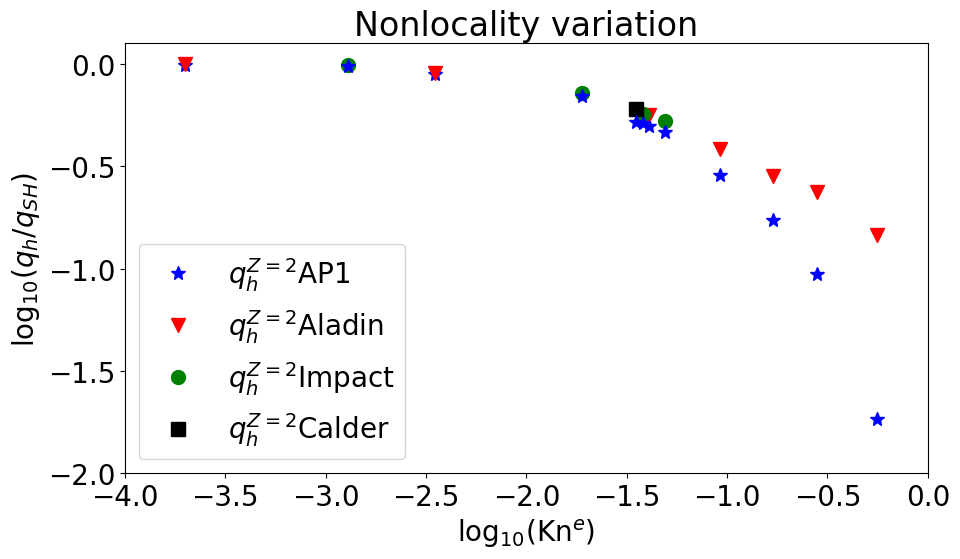
\includegraphics[width=0.5\textwidth]{Kn_results.png}
    \end{tabular}
  \caption{  
  Simulation results for the case $Z=2$ computed by AP1/Aladin/Impact/Calder.
  Every point corresponds to the maximum heat flux in a "tanh" temperature 
  simulation, which can be characterized by Kn. The range of 
  $\log_{10}(\text{Kn})\in (0, -4)$ can be expressed as equivalent 
  to the~electron density approximate range n$_e \in (1e19, 3.5e22)$ of 
  the~50 $\mu$m slope tanh case. In the case of Kn = 0.56, 
  $q_{Aladin} / q_{AP1}\approx 7.9$.}
  \label{fig:Kn_results}
  \end{center} 
\end{figure}

\begin{figure}[tbh]
  \begin{center}
    \begin{tabular}{c}
      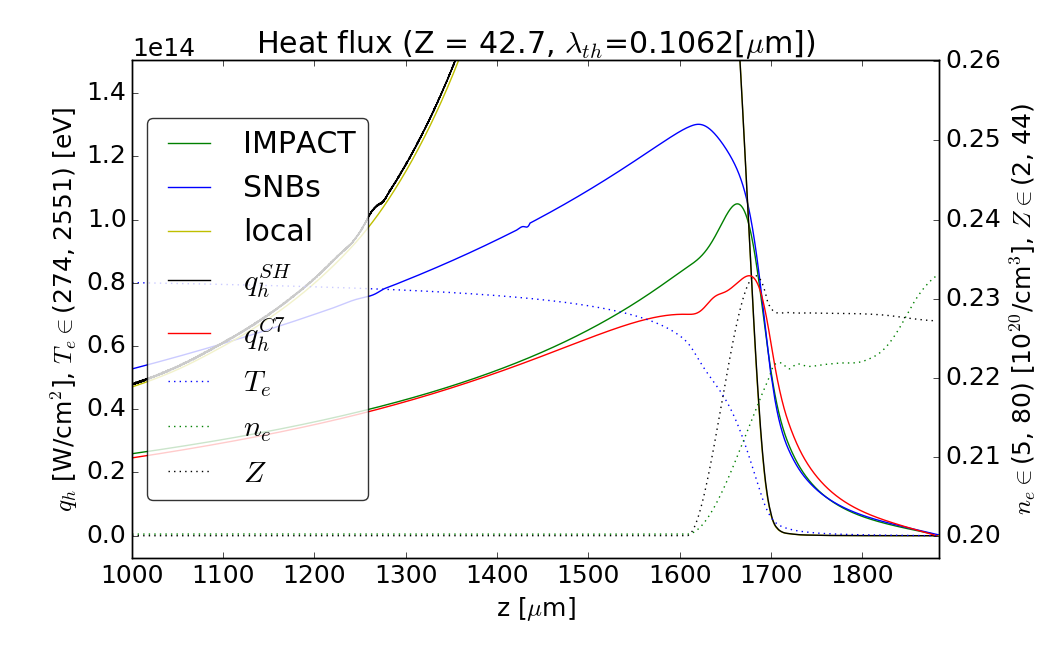
\includegraphics[width=0.5\textwidth]{../VFPdata/GD_Hohlraum/fluxes_10ps.png} 
    \end{tabular}
  \caption{
  }
  \label{fig:Gd_VFP_10ps_heatflux}
  \end{center} 
\end{figure}

\begin{itemize}
  \item Multiple runs analyzing the~performance of AP1 with respect to 
    Aladin/Impact/Calder along wide range of Kn$^e$ shown in 
    \figref{fig:Kn_results}.
  \item Realistic hydro simulation setting provided by HYDRA, a~comparison
    between AP1, Impact, and SNB shown in \figref{fig:Gd_VFP_10ps_heatflux}.
  \item Comment on and summarize the~velocity limits for all figs.
\end{itemize}

%
